
%(BEGIN_QUESTION)
% Copyright 2013, Tony R. Kuphaldt, released under the Creative Commons Attribution License (v 1.0)
% This means you may do almost anything with this work of mine, so long as you give me proper credit

This temperature control system has a problem.  The furnace is cold according to the operator who checked it personally, and the indicating controller (TIC) shows that the furnace temperature is near ambient temperature (85 $^{o}$F) while the setpoint is set to 1000 $^{o}$F.  A voltmeter connected between the ``+'' and ``$-$'' terminals on TY-205b registers 3.5 VDC:

$$\includegraphics[width=15.5cm]{i02827x01.eps}$$

Identify the likelihood of each specified fault for this circuit.  Consider each fault one at a time (i.e. no coincidental faults), determining whether or not each fault could independently account for {\it all} measurements and symptoms in this circuit.

% No blank lines allowed between lines of an \halign structure!
% I use comments (%) instead, so that TeX doesn't choke.

$$\vbox{\offinterlineskip
\halign{\strut
\vrule \quad\hfil # \ \hfil & 
\vrule \quad\hfil # \ \hfil & 
\vrule \quad\hfil # \ \hfil \vrule \cr
\noalign{\hrule}
%
% First row
{\bf Fault} & {\bf Possible} & {\bf Impossible} \cr
%
\noalign{\hrule}
%
% Another row
TY-205a failed open &  &  \cr
%
\noalign{\hrule}
%
% Another row
TY-205b failed open &  &  \cr
%
\noalign{\hrule}
%
% Another row
Cable TT-205 failed shorted &  &  \cr
%
\noalign{\hrule}
%
% Another row
Wire open between terminal 6 and terminal 9 &  &  \cr
%
\noalign{\hrule}
%
% Another row
Wire open between terminal 1 and terminal 7 &  &  \cr
%
\noalign{\hrule}
%
% Another row
Valve \#15 at column \#8 shut off &  &  \cr
%
\noalign{\hrule}
%
% Another row
Breaker \#4 at panel L2 tripped (off) &  &  \cr
%
\noalign{\hrule}
} % End of \halign 
}$$ % End of \vbox


\underbar{file i02827}
%(END_QUESTION)





%(BEGIN_ANSWER)

% No blank lines allowed between lines of an \halign structure!
% I use comments (%) instead, so that TeX doesn't choke.

$$\vbox{\offinterlineskip
\halign{\strut
\vrule \quad\hfil # \ \hfil & 
\vrule \quad\hfil # \ \hfil & 
\vrule \quad\hfil # \ \hfil \vrule \cr
\noalign{\hrule}
%
% First row
{\bf Fault} & {\bf Possible} & {\bf Impossible} \cr
%
\noalign{\hrule}
%
% Another row
TY-205a failed open &  & $\surd$ \cr
%
\noalign{\hrule}
%
% Another row
TY-205b failed open &  & $\surd$ \cr
%
\noalign{\hrule}
%
% Another row
Cable TT-205 failed shorted &  & $\surd$ \cr
%
\noalign{\hrule}
%
% Another row
Wire open between terminal 6 and terminal 9 &  & $\surd$ \cr
%
\noalign{\hrule}
%
% Another row
Wire open between terminal 1 and terminal 7 &  & $\surd$ \cr
%
\noalign{\hrule}
%
% Another row
Valve \#15 at column \#8 shut off & $\surd$ &  \cr
%
\noalign{\hrule}
%
% Another row
Breaker \#4 at panel L2 tripped (off) &  & $\surd$ \cr
%
\noalign{\hrule}
} % End of \halign 
}$$ % End of \vbox


%(END_ANSWER)





%(BEGIN_NOTES)

{\bf This question is intended for exams only and not worksheets!}.

%(END_NOTES)


